\documentclass[convert={outfile=\jobname.png}]{standalone}
\usepackage{base}

\begin{document}

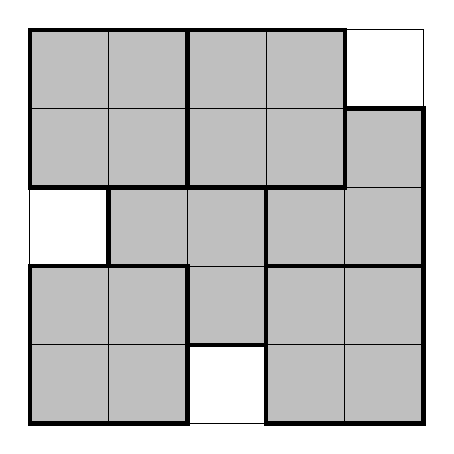
\begin{tikzpicture}[border/.style={fill=gray!50, ultra thick}]
    \def\n{5}
    \foreach \i/\j in {0/0, 0/3, 3/0, 2/3}
        \draw[border] (\i, \j) rectangle (\i + 2, \j + 2);
    \draw[border] (1, 3) --++ (2, 0) --++ (0, -2) --++ (-1, 0) --++ (0, 1) --++ (-1, 0) -- cycle;
    \draw[border] (3, 2) --++ (2, 0) --++ (0, 2) --++ (-1, 0) --++ (0, -1) --++ (-1, 0) -- cycle;
    \foreach \i in {0, ..., \n} {
        \draw (\i, 0) -- (\i, \n);
        \draw (0, \i) -- (\n, \i);
    }
\end{tikzpicture}

\end{document}
